%\documentclass[11pt,a4paper]{article}
%\usepackage{polski}
%\usepackage[utf8]{inputenc}
%\usepackage{graphicx}

\title{Projektowanie algorytmów i metod sztucznej inteligencji\\Laboratorium  8- Sprawozdanie}
\author{Wojciech Makuch}
\date{}

%\begin{document}
	\maketitle
	\section{Zadanie}\label{sec:Zadanie}
	Implementacja drzewa binarnego oraz drzewa czerwono-czarnego. Zbadanie złożoności obliczeniowej metody wstawiania oraz przeszukiwania.
	
	\section{Wstep}\label{sec:Wstep}
	Binarne drzewo przeszukiwań – struktura danych przechowująca dane oraz 2 wskaźniki na elementy następne zwane prawym oraz lewym synem. Koszt wykonania podstawowych operacji w drzewie BST jest proporcjonalny do wysokości drzewa h, ponieważ operacje wykonywane są wzdłuż drzewa. Jeżeli drzewo jest zrównoważone, to jego wysokość bliska jest logarytmowi dwójkowemu liczby węzłów. Złożoność obliczeniowa wynosi wtedy $O(log_{2}n)$. Z drugiej strony drzewo skrajnie niezrównoważone ma wysokość porównywalną z liczbą węzłów (w skrajnym przypadku drzewa zdegenerowanego do listy wartości te są równe: h=n), z tego powodu koszt pesymistyczny wzrasta do $O(n)$. 
	
	\section{Drzewo binarne - implementacja}\label{sec:Drzewo binarne - implementacja}
	Utworzono klasę węzła posiadającą wskaźniki na ojca, lewego syna i prawego syna oraz klasę drzewa składającego się z węzłów przechowującą wskaźnik na korzeń. Zaimplementowano podstawowe metody takie jak dodawanie elementu zgodnie z zasadą drzewa binarnego, wyświetlanie zawartości drzewa zgodnie z metodą preorder oraz przeszukiwanie drzewa w celu znalezienia węzła o zadanym kluczy. Ponadto klasa jest obserwowana przez klasę benchmarkujące oraz posiada metody zawieracjące pętle benchmarkujące.  
	
	\section{Drzewo czerowno-czarne}\label{sec:Drzewo czerowno-czarne}
Drzewo czerwono-czarne – drzewo binarne dążące do zrównoważenie się, dzięki czemu głębokość jest mniejsza niż w zwykłym drzewie binarnym. Zachowuje własności:
\begin{enumerate}
\item	Każdy węzeł jest czerwony lub czarny.
\item	Korzeń jest czarny.
\item	Każdy liść jest czarny (Można traktować nil jako liść).
\item	Jeśli węzeł jest czerwony, to jego synowie muszą być czarni.
\item	Każda ścieżka z ustalonego węzła do liścia liczy tyle samo czarnych węzłów
\end{enumerate}
	
	\section{Drzewa czerwono-czarne - implementacja}\label{sec:Drzewa czerwono-czarne - implementacja}
	Implementacje drzewa czerwono – czarnego wykonano analogicznie do drzewa binarnego. Klasa węzeł zawiera dodatkowe pole informujące o kolorze. Ponadto zastosowano wartownika informujący kiedy następują liście nie przechowujące żadnej wartości. Zaimplementowano metody rotacji w prawo oraz rotacji w lewo w wykorzystane w metodzie dodawania elementów, aby zrównoważyć drzewo. Metoda wstawiania elementu do drzewa czerwono – czarnego jest rozbudowaniem metody wstawiania do zwykłego drzewa binarnego sprawdzająca 5 przypadków i wykonująca następujące kroki:
	\begin{enumerate}
	\item Gdy ojciec i wuj sa czerwoni, zmien ich kolory.
	\item Gdy lewy ojeciec i jego lewy syn sa czeroni, wykonaj obrot w prawo dziadka i ojca oraz zamien ich kolory.
	\item Gdy lewy ojciec i jego prawy syn sa czerwoni, wykonaj obrot w lewo ojca i syna oraz wykonaj 2).
	\item Gdy prawy ojciec i jego prawy syn sa czerwoni, wykonaj obrot w lewo  dziadka i ojca, zamien ich kolory
	\item Gdy prawy ojciec i jego prawy syn sa czerwoni, wykonaj obrot w prawo ojca i syna oraz wykonaj 4)
	\end{enumerate}
	Ponadto klasa zawiera metody benchmarkujące analogicznie jak w drzewie binarnym.
	
	\section{Zlozonosci obliczeniowe usyskane}\label{sec:Zlozonosci obliczeniowe usyskane}
	Na rysunkach poniżej przedstawiono uzyskane wyniki złożoność obliczeniowych. Analizując je po kolei można dojść do wniosku, że wstawiania do drzewa binarnego ma pesymistyczną złożoność obliczeniowa $O(n)$. Wykres nieco ucieka od tej wartości, co może być spowodowane niedokładną implementacją algorytmu(np. brak wartownika przy zwykłym drzewie binarnym). Najlepsze wyniki dają algorytmy wyszukiwania w drzewie binarnym oraz binarnym czerwono –czarnym, ponieważ tam działają tylko operatory porównania. Uzyskana złożoność obliczeniowa wynosi $O(log_{2}n)$, w przypadku pesymistycznym $O(n)$. Algorytm wstawiania do drzewa czerwono-czarnego ma posiada lepszą złożoność obliczeniową, niż w przypadku zwykłego drzewa binarnego, ale wynosi ona w przypadku pesymistycznym również $O(n)$.
	\begin{figure}
	\centering
	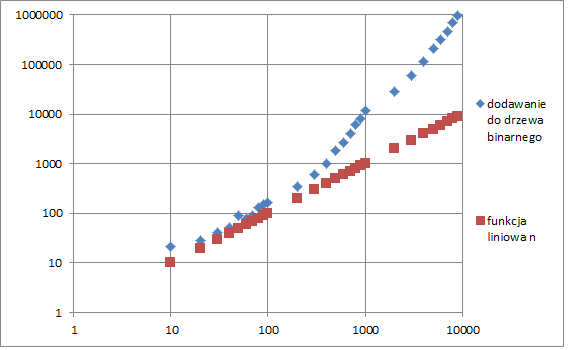
\includegraphics[scale=0.9]{1.png}
	\caption{Dodawanie do drzewa binarnego.}
	\label{fig:1}
	\end{figure}
	\begin{figure}
	\centering
	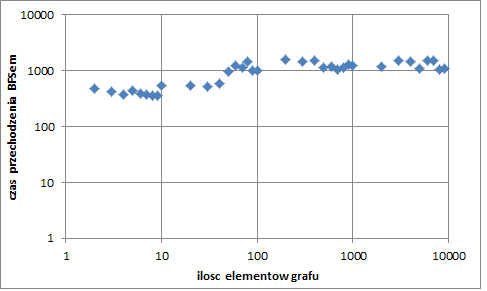
\includegraphics[scale=0.90]{2.png}
	\caption{Prszeszukiwanie drzewa binarnego.}
	\label{fig:2}
	\end{figure}
	\begin{figure}
	\centering
	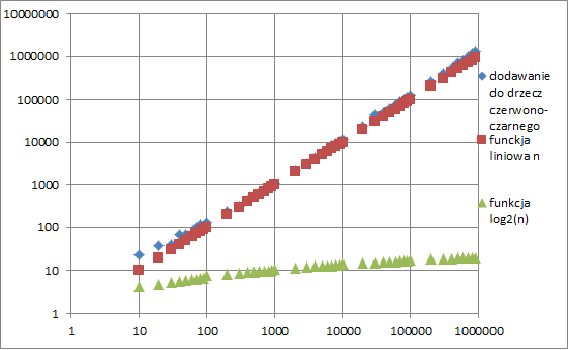
\includegraphics[scale=0.9]{3.png}
	\caption{Dodawanie do drzewa czerwono-czarnego.}
	\label{fig:3}
	\end{figure}
	\begin{figure}
	\centering
	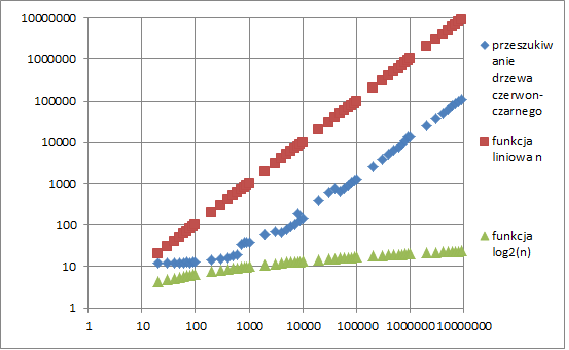
\includegraphics[scale=0.9]{4.png}
	\caption{Przeszukiwanie drzewa czerwono-czarnego.}
	\label{fig:4}
	\end{figure}
	\section{Komentarz}\label{sec:Komentarz}
	Do utworzenia dokumentacji wykorzystano system Doxygen. Funkcja pomiaru czasu dla systemu Windows pobrana ze strony dr. J. Mierzwy. Program skompilowano w środowisku Code::Blocks. Do stworzenia wykresu posłużono się pakietem MS Excel, sprawozdanie napisano używając systemu \LaTeX.

\end{document}
